\documentclass[14pt,letterpaper]{extarticle}
\usepackage[letterpaper,left=0.7in,right=0.7in,top=0.85in,bottom=0.85in,headheight=18pt,headsep=14pt,footskip=0.45in]{geometry}
\usepackage[T1]{fontenc}
\usepackage{newcent}
\usepackage{tikz}
\usepackage{array}
\usepackage{fancyhdr}
\pagestyle{fancy}
\fancyhf{}
\fancyhead[L]{Week 7 / Take-away games / Grades K--1}
\fancyfoot[L]{Bellingham Math Circle / Week 7}
\fancyfoot[R]{\thepage}
\renewcommand{\headrulewidth}{0.4pt}
\renewcommand{\footrulewidth}{0pt}
\setlength{\parindent}{0pt}
\setlength{\parskip}{0pt}
\hyphenpenalty=10000
\exhyphenpenalty=10000
\setlength{\emergencystretch}{3em}
\newcommand{\prob}[1]{\textbf{Problem #1:}}
\newcommand{\game}[1]{\mbox{\{#1\}}}
\newenvironment{problem}{\par\noindent\begin{minipage}{\linewidth}}{\end{minipage}\par\vspace{0.9cm}}
\begin{document}
Two players take turns taking counters. Unless a problem says something else, a player takes 1 or 2 counters on each turn, and whoever takes the last counter wins.

\vspace{0.7cm}
\begin{problem}
\prob{1} On your turn, circle the counters you take to be sure to win. Cross out each pile where you cannot be sure to win.
\begin{center}
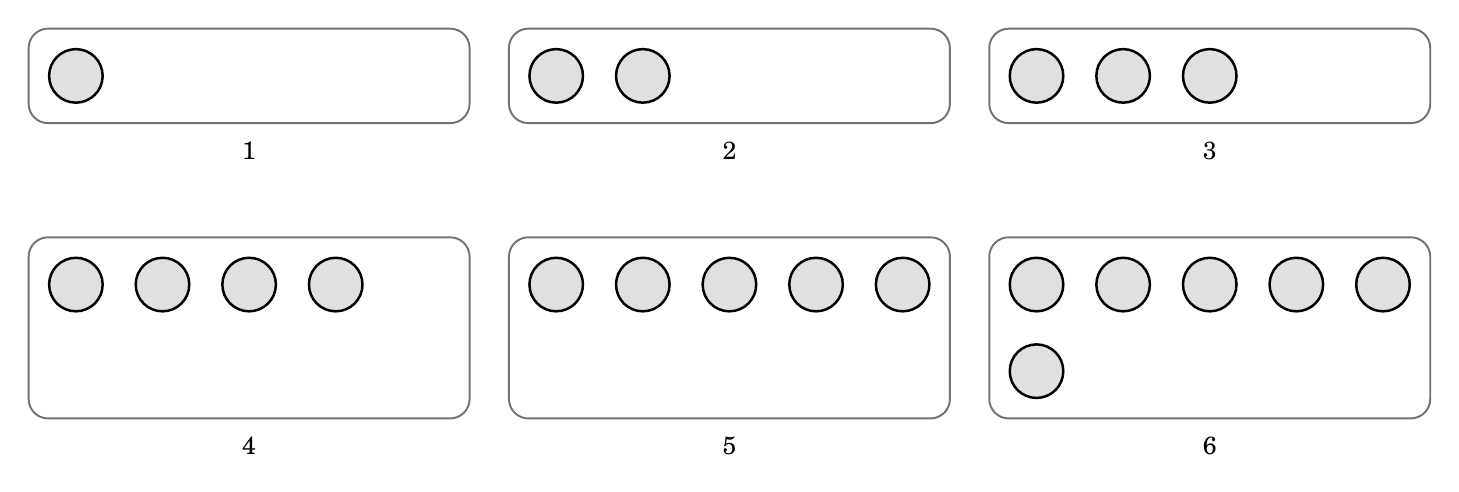
\begin{tikzpicture}
\draw[black!55,line width=0.7pt,rounded corners=7pt] (0.000,0.000) rectangle (5.600,-1.200);
\draw[fill=black!12,line width=0.9pt] (0.600,-0.600) circle (0.34);
\node[font=\small] at (2.800,-1.550) {1};
\draw[black!55,line width=0.7pt,rounded corners=7pt] (6.100,0.000) rectangle (11.700,-1.200);
\draw[fill=black!12,line width=0.9pt] (6.700,-0.600) circle (0.34);
\draw[fill=black!12,line width=0.9pt] (7.800,-0.600) circle (0.34);
\node[font=\small] at (8.900,-1.550) {2};
\draw[black!55,line width=0.7pt,rounded corners=7pt] (12.200,0.000) rectangle (17.800,-1.200);
\draw[fill=black!12,line width=0.9pt] (12.800,-0.600) circle (0.34);
\draw[fill=black!12,line width=0.9pt] (13.900,-0.600) circle (0.34);
\draw[fill=black!12,line width=0.9pt] (15.000,-0.600) circle (0.34);
\node[font=\small] at (15.000,-1.550) {3};
\draw[black!55,line width=0.7pt,rounded corners=7pt] (0.000,-2.650) rectangle (5.600,-4.950);
\draw[fill=black!12,line width=0.9pt] (0.600,-3.250) circle (0.34);
\draw[fill=black!12,line width=0.9pt] (1.700,-3.250) circle (0.34);
\draw[fill=black!12,line width=0.9pt] (2.800,-3.250) circle (0.34);
\draw[fill=black!12,line width=0.9pt] (3.900,-3.250) circle (0.34);
\node[font=\small] at (2.800,-5.300) {4};
\draw[black!55,line width=0.7pt,rounded corners=7pt] (6.100,-2.650) rectangle (11.700,-4.950);
\draw[fill=black!12,line width=0.9pt] (6.700,-3.250) circle (0.34);
\draw[fill=black!12,line width=0.9pt] (7.800,-3.250) circle (0.34);
\draw[fill=black!12,line width=0.9pt] (8.900,-3.250) circle (0.34);
\draw[fill=black!12,line width=0.9pt] (10.000,-3.250) circle (0.34);
\draw[fill=black!12,line width=0.9pt] (11.100,-3.250) circle (0.34);
\node[font=\small] at (8.900,-5.300) {5};
\draw[black!55,line width=0.7pt,rounded corners=7pt] (12.200,-2.650) rectangle (17.800,-4.950);
\draw[fill=black!12,line width=0.9pt] (12.800,-3.250) circle (0.34);
\draw[fill=black!12,line width=0.9pt] (13.900,-3.250) circle (0.34);
\draw[fill=black!12,line width=0.9pt] (15.000,-3.250) circle (0.34);
\draw[fill=black!12,line width=0.9pt] (16.100,-3.250) circle (0.34);
\draw[fill=black!12,line width=0.9pt] (17.200,-3.250) circle (0.34);
\draw[fill=black!12,line width=0.9pt] (12.800,-4.350) circle (0.34);
\node[font=\small] at (15.000,-5.300) {6};
\end{tikzpicture}
\end{center}

\end{problem}
\begin{problem}
\prob{2} Would you rather go 1st or 2nd with each pile? Circle 1st or 2nd.
\begin{center}
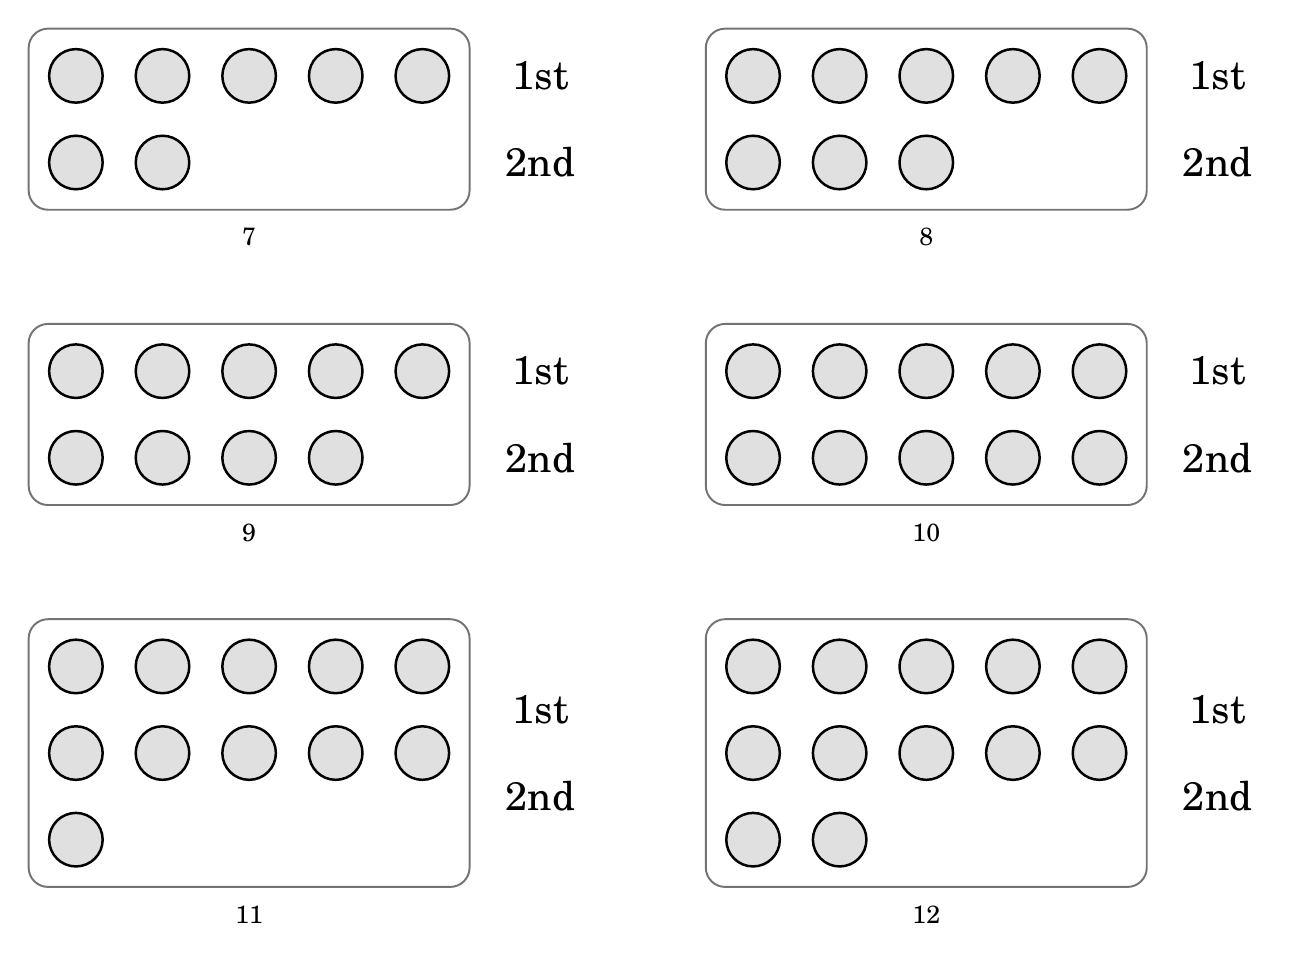
\begin{tikzpicture}
\draw[black!55,line width=0.7pt,rounded corners=7pt] (0.000,0.000) rectangle (5.600,-2.300);
\draw[fill=black!12,line width=0.9pt] (0.600,-0.600) circle (0.34);
\draw[fill=black!12,line width=0.9pt] (1.700,-0.600) circle (0.34);
\draw[fill=black!12,line width=0.9pt] (2.800,-0.600) circle (0.34);
\draw[fill=black!12,line width=0.9pt] (3.900,-0.600) circle (0.34);
\draw[fill=black!12,line width=0.9pt] (5.000,-0.600) circle (0.34);
\draw[fill=black!12,line width=0.9pt] (0.600,-1.700) circle (0.34);
\draw[fill=black!12,line width=0.9pt] (1.700,-1.700) circle (0.34);
\node[font=\Large] at (6.500,-0.600) {1st};
\node[font=\Large] at (6.500,-1.700) {2nd};
\node[font=\small] at (2.800,-2.650) {7};
\draw[black!55,line width=0.7pt,rounded corners=7pt] (8.600,0.000) rectangle (14.200,-2.300);
\draw[fill=black!12,line width=0.9pt] (9.200,-0.600) circle (0.34);
\draw[fill=black!12,line width=0.9pt] (10.300,-0.600) circle (0.34);
\draw[fill=black!12,line width=0.9pt] (11.400,-0.600) circle (0.34);
\draw[fill=black!12,line width=0.9pt] (12.500,-0.600) circle (0.34);
\draw[fill=black!12,line width=0.9pt] (13.600,-0.600) circle (0.34);
\draw[fill=black!12,line width=0.9pt] (9.200,-1.700) circle (0.34);
\draw[fill=black!12,line width=0.9pt] (10.300,-1.700) circle (0.34);
\draw[fill=black!12,line width=0.9pt] (11.400,-1.700) circle (0.34);
\node[font=\Large] at (15.100,-0.600) {1st};
\node[font=\Large] at (15.100,-1.700) {2nd};
\node[font=\small] at (11.400,-2.650) {8};
\draw[black!55,line width=0.7pt,rounded corners=7pt] (0.000,-3.750) rectangle (5.600,-6.050);
\draw[fill=black!12,line width=0.9pt] (0.600,-4.350) circle (0.34);
\draw[fill=black!12,line width=0.9pt] (1.700,-4.350) circle (0.34);
\draw[fill=black!12,line width=0.9pt] (2.800,-4.350) circle (0.34);
\draw[fill=black!12,line width=0.9pt] (3.900,-4.350) circle (0.34);
\draw[fill=black!12,line width=0.9pt] (5.000,-4.350) circle (0.34);
\draw[fill=black!12,line width=0.9pt] (0.600,-5.450) circle (0.34);
\draw[fill=black!12,line width=0.9pt] (1.700,-5.450) circle (0.34);
\draw[fill=black!12,line width=0.9pt] (2.800,-5.450) circle (0.34);
\draw[fill=black!12,line width=0.9pt] (3.900,-5.450) circle (0.34);
\node[font=\Large] at (6.500,-4.350) {1st};
\node[font=\Large] at (6.500,-5.450) {2nd};
\node[font=\small] at (2.800,-6.400) {9};
\draw[black!55,line width=0.7pt,rounded corners=7pt] (8.600,-3.750) rectangle (14.200,-6.050);
\draw[fill=black!12,line width=0.9pt] (9.200,-4.350) circle (0.34);
\draw[fill=black!12,line width=0.9pt] (10.300,-4.350) circle (0.34);
\draw[fill=black!12,line width=0.9pt] (11.400,-4.350) circle (0.34);
\draw[fill=black!12,line width=0.9pt] (12.500,-4.350) circle (0.34);
\draw[fill=black!12,line width=0.9pt] (13.600,-4.350) circle (0.34);
\draw[fill=black!12,line width=0.9pt] (9.200,-5.450) circle (0.34);
\draw[fill=black!12,line width=0.9pt] (10.300,-5.450) circle (0.34);
\draw[fill=black!12,line width=0.9pt] (11.400,-5.450) circle (0.34);
\draw[fill=black!12,line width=0.9pt] (12.500,-5.450) circle (0.34);
\draw[fill=black!12,line width=0.9pt] (13.600,-5.450) circle (0.34);
\node[font=\Large] at (15.100,-4.350) {1st};
\node[font=\Large] at (15.100,-5.450) {2nd};
\node[font=\small] at (11.400,-6.400) {10};
\draw[black!55,line width=0.7pt,rounded corners=7pt] (0.000,-7.500) rectangle (5.600,-10.900);
\draw[fill=black!12,line width=0.9pt] (0.600,-8.100) circle (0.34);
\draw[fill=black!12,line width=0.9pt] (1.700,-8.100) circle (0.34);
\draw[fill=black!12,line width=0.9pt] (2.800,-8.100) circle (0.34);
\draw[fill=black!12,line width=0.9pt] (3.900,-8.100) circle (0.34);
\draw[fill=black!12,line width=0.9pt] (5.000,-8.100) circle (0.34);
\draw[fill=black!12,line width=0.9pt] (0.600,-9.200) circle (0.34);
\draw[fill=black!12,line width=0.9pt] (1.700,-9.200) circle (0.34);
\draw[fill=black!12,line width=0.9pt] (2.800,-9.200) circle (0.34);
\draw[fill=black!12,line width=0.9pt] (3.900,-9.200) circle (0.34);
\draw[fill=black!12,line width=0.9pt] (5.000,-9.200) circle (0.34);
\draw[fill=black!12,line width=0.9pt] (0.600,-10.300) circle (0.34);
\node[font=\Large] at (6.500,-8.650) {1st};
\node[font=\Large] at (6.500,-9.750) {2nd};
\node[font=\small] at (2.800,-11.250) {11};
\draw[black!55,line width=0.7pt,rounded corners=7pt] (8.600,-7.500) rectangle (14.200,-10.900);
\draw[fill=black!12,line width=0.9pt] (9.200,-8.100) circle (0.34);
\draw[fill=black!12,line width=0.9pt] (10.300,-8.100) circle (0.34);
\draw[fill=black!12,line width=0.9pt] (11.400,-8.100) circle (0.34);
\draw[fill=black!12,line width=0.9pt] (12.500,-8.100) circle (0.34);
\draw[fill=black!12,line width=0.9pt] (13.600,-8.100) circle (0.34);
\draw[fill=black!12,line width=0.9pt] (9.200,-9.200) circle (0.34);
\draw[fill=black!12,line width=0.9pt] (10.300,-9.200) circle (0.34);
\draw[fill=black!12,line width=0.9pt] (11.400,-9.200) circle (0.34);
\draw[fill=black!12,line width=0.9pt] (12.500,-9.200) circle (0.34);
\draw[fill=black!12,line width=0.9pt] (13.600,-9.200) circle (0.34);
\draw[fill=black!12,line width=0.9pt] (9.200,-10.300) circle (0.34);
\draw[fill=black!12,line width=0.9pt] (10.300,-10.300) circle (0.34);
\node[font=\Large] at (15.100,-8.650) {1st};
\node[font=\Large] at (15.100,-9.750) {2nd};
\node[font=\small] at (11.400,-11.250) {12};
\end{tikzpicture}
\end{center}

\end{problem}
\begin{problem}
\prob{3} A trap is a pile you do not want to have on your turn. Put an X on every trap from 1 to 20.
\begin{center}
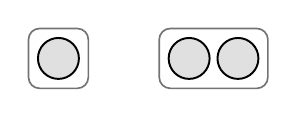
\begin{tikzpicture}
\draw[black!55,line width=0.6pt,rounded corners=4pt] (0.000,0) rectangle (0.760,-0.760);
\draw[fill=black!12,line width=0.7pt] (0.380,-0.380) circle (0.26);
\draw[black!55,line width=0.6pt,rounded corners=4pt] (1.660,0) rectangle (3.040,-0.760);
\draw[fill=black!12,line width=0.7pt] (2.040,-0.380) circle (0.26);
\draw[fill=black!12,line width=0.7pt] (2.660,-0.380) circle (0.26);
\end{tikzpicture}
\end{center}
\vspace{-0.1cm}
\begin{center}
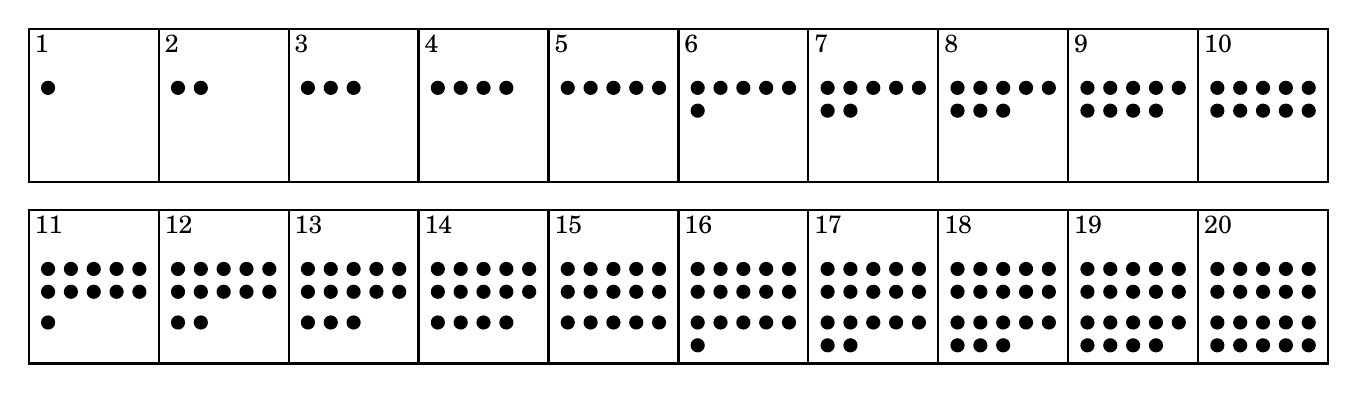
\begin{tikzpicture}
\draw[line width=0.8pt] (0.000,0.000) rectangle (1.650,-1.950);
\node[font=\small,anchor=north west,inner sep=2pt] at (0.000,0.000) {1};
\fill (0.245,-0.750) circle (0.09);
\draw[line width=0.8pt] (1.650,0.000) rectangle (3.300,-1.950);
\node[font=\small,anchor=north west,inner sep=2pt] at (1.650,0.000) {2};
\fill (1.895,-0.750) circle (0.09);
\fill (2.185,-0.750) circle (0.09);
\draw[line width=0.8pt] (3.300,0.000) rectangle (4.950,-1.950);
\node[font=\small,anchor=north west,inner sep=2pt] at (3.300,0.000) {3};
\fill (3.545,-0.750) circle (0.09);
\fill (3.835,-0.750) circle (0.09);
\fill (4.125,-0.750) circle (0.09);
\draw[line width=0.8pt] (4.950,0.000) rectangle (6.600,-1.950);
\node[font=\small,anchor=north west,inner sep=2pt] at (4.950,0.000) {4};
\fill (5.195,-0.750) circle (0.09);
\fill (5.485,-0.750) circle (0.09);
\fill (5.775,-0.750) circle (0.09);
\fill (6.065,-0.750) circle (0.09);
\draw[line width=0.8pt] (6.600,0.000) rectangle (8.250,-1.950);
\node[font=\small,anchor=north west,inner sep=2pt] at (6.600,0.000) {5};
\fill (6.845,-0.750) circle (0.09);
\fill (7.135,-0.750) circle (0.09);
\fill (7.425,-0.750) circle (0.09);
\fill (7.715,-0.750) circle (0.09);
\fill (8.005,-0.750) circle (0.09);
\draw[line width=0.8pt] (8.250,0.000) rectangle (9.900,-1.950);
\node[font=\small,anchor=north west,inner sep=2pt] at (8.250,0.000) {6};
\fill (8.495,-0.750) circle (0.09);
\fill (8.785,-0.750) circle (0.09);
\fill (9.075,-0.750) circle (0.09);
\fill (9.365,-0.750) circle (0.09);
\fill (9.655,-0.750) circle (0.09);
\fill (8.495,-1.040) circle (0.09);
\draw[line width=0.8pt] (9.900,0.000) rectangle (11.550,-1.950);
\node[font=\small,anchor=north west,inner sep=2pt] at (9.900,0.000) {7};
\fill (10.145,-0.750) circle (0.09);
\fill (10.435,-0.750) circle (0.09);
\fill (10.725,-0.750) circle (0.09);
\fill (11.015,-0.750) circle (0.09);
\fill (11.305,-0.750) circle (0.09);
\fill (10.145,-1.040) circle (0.09);
\fill (10.435,-1.040) circle (0.09);
\draw[line width=0.8pt] (11.550,0.000) rectangle (13.200,-1.950);
\node[font=\small,anchor=north west,inner sep=2pt] at (11.550,0.000) {8};
\fill (11.795,-0.750) circle (0.09);
\fill (12.085,-0.750) circle (0.09);
\fill (12.375,-0.750) circle (0.09);
\fill (12.665,-0.750) circle (0.09);
\fill (12.955,-0.750) circle (0.09);
\fill (11.795,-1.040) circle (0.09);
\fill (12.085,-1.040) circle (0.09);
\fill (12.375,-1.040) circle (0.09);
\draw[line width=0.8pt] (13.200,0.000) rectangle (14.850,-1.950);
\node[font=\small,anchor=north west,inner sep=2pt] at (13.200,0.000) {9};
\fill (13.445,-0.750) circle (0.09);
\fill (13.735,-0.750) circle (0.09);
\fill (14.025,-0.750) circle (0.09);
\fill (14.315,-0.750) circle (0.09);
\fill (14.605,-0.750) circle (0.09);
\fill (13.445,-1.040) circle (0.09);
\fill (13.735,-1.040) circle (0.09);
\fill (14.025,-1.040) circle (0.09);
\fill (14.315,-1.040) circle (0.09);
\draw[line width=0.8pt] (14.850,0.000) rectangle (16.500,-1.950);
\node[font=\small,anchor=north west,inner sep=2pt] at (14.850,0.000) {10};
\fill (15.095,-0.750) circle (0.09);
\fill (15.385,-0.750) circle (0.09);
\fill (15.675,-0.750) circle (0.09);
\fill (15.965,-0.750) circle (0.09);
\fill (16.255,-0.750) circle (0.09);
\fill (15.095,-1.040) circle (0.09);
\fill (15.385,-1.040) circle (0.09);
\fill (15.675,-1.040) circle (0.09);
\fill (15.965,-1.040) circle (0.09);
\fill (16.255,-1.040) circle (0.09);
\draw[line width=0.8pt] (0.000,-2.300) rectangle (1.650,-4.250);
\node[font=\small,anchor=north west,inner sep=2pt] at (0.000,-2.300) {11};
\fill (0.245,-3.050) circle (0.09);
\fill (0.535,-3.050) circle (0.09);
\fill (0.825,-3.050) circle (0.09);
\fill (1.115,-3.050) circle (0.09);
\fill (1.405,-3.050) circle (0.09);
\fill (0.245,-3.340) circle (0.09);
\fill (0.535,-3.340) circle (0.09);
\fill (0.825,-3.340) circle (0.09);
\fill (1.115,-3.340) circle (0.09);
\fill (1.405,-3.340) circle (0.09);
\fill (0.245,-3.730) circle (0.09);
\draw[line width=0.8pt] (1.650,-2.300) rectangle (3.300,-4.250);
\node[font=\small,anchor=north west,inner sep=2pt] at (1.650,-2.300) {12};
\fill (1.895,-3.050) circle (0.09);
\fill (2.185,-3.050) circle (0.09);
\fill (2.475,-3.050) circle (0.09);
\fill (2.765,-3.050) circle (0.09);
\fill (3.055,-3.050) circle (0.09);
\fill (1.895,-3.340) circle (0.09);
\fill (2.185,-3.340) circle (0.09);
\fill (2.475,-3.340) circle (0.09);
\fill (2.765,-3.340) circle (0.09);
\fill (3.055,-3.340) circle (0.09);
\fill (1.895,-3.730) circle (0.09);
\fill (2.185,-3.730) circle (0.09);
\draw[line width=0.8pt] (3.300,-2.300) rectangle (4.950,-4.250);
\node[font=\small,anchor=north west,inner sep=2pt] at (3.300,-2.300) {13};
\fill (3.545,-3.050) circle (0.09);
\fill (3.835,-3.050) circle (0.09);
\fill (4.125,-3.050) circle (0.09);
\fill (4.415,-3.050) circle (0.09);
\fill (4.705,-3.050) circle (0.09);
\fill (3.545,-3.340) circle (0.09);
\fill (3.835,-3.340) circle (0.09);
\fill (4.125,-3.340) circle (0.09);
\fill (4.415,-3.340) circle (0.09);
\fill (4.705,-3.340) circle (0.09);
\fill (3.545,-3.730) circle (0.09);
\fill (3.835,-3.730) circle (0.09);
\fill (4.125,-3.730) circle (0.09);
\draw[line width=0.8pt] (4.950,-2.300) rectangle (6.600,-4.250);
\node[font=\small,anchor=north west,inner sep=2pt] at (4.950,-2.300) {14};
\fill (5.195,-3.050) circle (0.09);
\fill (5.485,-3.050) circle (0.09);
\fill (5.775,-3.050) circle (0.09);
\fill (6.065,-3.050) circle (0.09);
\fill (6.355,-3.050) circle (0.09);
\fill (5.195,-3.340) circle (0.09);
\fill (5.485,-3.340) circle (0.09);
\fill (5.775,-3.340) circle (0.09);
\fill (6.065,-3.340) circle (0.09);
\fill (6.355,-3.340) circle (0.09);
\fill (5.195,-3.730) circle (0.09);
\fill (5.485,-3.730) circle (0.09);
\fill (5.775,-3.730) circle (0.09);
\fill (6.065,-3.730) circle (0.09);
\draw[line width=0.8pt] (6.600,-2.300) rectangle (8.250,-4.250);
\node[font=\small,anchor=north west,inner sep=2pt] at (6.600,-2.300) {15};
\fill (6.845,-3.050) circle (0.09);
\fill (7.135,-3.050) circle (0.09);
\fill (7.425,-3.050) circle (0.09);
\fill (7.715,-3.050) circle (0.09);
\fill (8.005,-3.050) circle (0.09);
\fill (6.845,-3.340) circle (0.09);
\fill (7.135,-3.340) circle (0.09);
\fill (7.425,-3.340) circle (0.09);
\fill (7.715,-3.340) circle (0.09);
\fill (8.005,-3.340) circle (0.09);
\fill (6.845,-3.730) circle (0.09);
\fill (7.135,-3.730) circle (0.09);
\fill (7.425,-3.730) circle (0.09);
\fill (7.715,-3.730) circle (0.09);
\fill (8.005,-3.730) circle (0.09);
\draw[line width=0.8pt] (8.250,-2.300) rectangle (9.900,-4.250);
\node[font=\small,anchor=north west,inner sep=2pt] at (8.250,-2.300) {16};
\fill (8.495,-3.050) circle (0.09);
\fill (8.785,-3.050) circle (0.09);
\fill (9.075,-3.050) circle (0.09);
\fill (9.365,-3.050) circle (0.09);
\fill (9.655,-3.050) circle (0.09);
\fill (8.495,-3.340) circle (0.09);
\fill (8.785,-3.340) circle (0.09);
\fill (9.075,-3.340) circle (0.09);
\fill (9.365,-3.340) circle (0.09);
\fill (9.655,-3.340) circle (0.09);
\fill (8.495,-3.730) circle (0.09);
\fill (8.785,-3.730) circle (0.09);
\fill (9.075,-3.730) circle (0.09);
\fill (9.365,-3.730) circle (0.09);
\fill (9.655,-3.730) circle (0.09);
\fill (8.495,-4.020) circle (0.09);
\draw[line width=0.8pt] (9.900,-2.300) rectangle (11.550,-4.250);
\node[font=\small,anchor=north west,inner sep=2pt] at (9.900,-2.300) {17};
\fill (10.145,-3.050) circle (0.09);
\fill (10.435,-3.050) circle (0.09);
\fill (10.725,-3.050) circle (0.09);
\fill (11.015,-3.050) circle (0.09);
\fill (11.305,-3.050) circle (0.09);
\fill (10.145,-3.340) circle (0.09);
\fill (10.435,-3.340) circle (0.09);
\fill (10.725,-3.340) circle (0.09);
\fill (11.015,-3.340) circle (0.09);
\fill (11.305,-3.340) circle (0.09);
\fill (10.145,-3.730) circle (0.09);
\fill (10.435,-3.730) circle (0.09);
\fill (10.725,-3.730) circle (0.09);
\fill (11.015,-3.730) circle (0.09);
\fill (11.305,-3.730) circle (0.09);
\fill (10.145,-4.020) circle (0.09);
\fill (10.435,-4.020) circle (0.09);
\draw[line width=0.8pt] (11.550,-2.300) rectangle (13.200,-4.250);
\node[font=\small,anchor=north west,inner sep=2pt] at (11.550,-2.300) {18};
\fill (11.795,-3.050) circle (0.09);
\fill (12.085,-3.050) circle (0.09);
\fill (12.375,-3.050) circle (0.09);
\fill (12.665,-3.050) circle (0.09);
\fill (12.955,-3.050) circle (0.09);
\fill (11.795,-3.340) circle (0.09);
\fill (12.085,-3.340) circle (0.09);
\fill (12.375,-3.340) circle (0.09);
\fill (12.665,-3.340) circle (0.09);
\fill (12.955,-3.340) circle (0.09);
\fill (11.795,-3.730) circle (0.09);
\fill (12.085,-3.730) circle (0.09);
\fill (12.375,-3.730) circle (0.09);
\fill (12.665,-3.730) circle (0.09);
\fill (12.955,-3.730) circle (0.09);
\fill (11.795,-4.020) circle (0.09);
\fill (12.085,-4.020) circle (0.09);
\fill (12.375,-4.020) circle (0.09);
\draw[line width=0.8pt] (13.200,-2.300) rectangle (14.850,-4.250);
\node[font=\small,anchor=north west,inner sep=2pt] at (13.200,-2.300) {19};
\fill (13.445,-3.050) circle (0.09);
\fill (13.735,-3.050) circle (0.09);
\fill (14.025,-3.050) circle (0.09);
\fill (14.315,-3.050) circle (0.09);
\fill (14.605,-3.050) circle (0.09);
\fill (13.445,-3.340) circle (0.09);
\fill (13.735,-3.340) circle (0.09);
\fill (14.025,-3.340) circle (0.09);
\fill (14.315,-3.340) circle (0.09);
\fill (14.605,-3.340) circle (0.09);
\fill (13.445,-3.730) circle (0.09);
\fill (13.735,-3.730) circle (0.09);
\fill (14.025,-3.730) circle (0.09);
\fill (14.315,-3.730) circle (0.09);
\fill (14.605,-3.730) circle (0.09);
\fill (13.445,-4.020) circle (0.09);
\fill (13.735,-4.020) circle (0.09);
\fill (14.025,-4.020) circle (0.09);
\fill (14.315,-4.020) circle (0.09);
\draw[line width=0.8pt] (14.850,-2.300) rectangle (16.500,-4.250);
\node[font=\small,anchor=north west,inner sep=2pt] at (14.850,-2.300) {20};
\fill (15.095,-3.050) circle (0.09);
\fill (15.385,-3.050) circle (0.09);
\fill (15.675,-3.050) circle (0.09);
\fill (15.965,-3.050) circle (0.09);
\fill (16.255,-3.050) circle (0.09);
\fill (15.095,-3.340) circle (0.09);
\fill (15.385,-3.340) circle (0.09);
\fill (15.675,-3.340) circle (0.09);
\fill (15.965,-3.340) circle (0.09);
\fill (16.255,-3.340) circle (0.09);
\fill (15.095,-3.730) circle (0.09);
\fill (15.385,-3.730) circle (0.09);
\fill (15.675,-3.730) circle (0.09);
\fill (15.965,-3.730) circle (0.09);
\fill (16.255,-3.730) circle (0.09);
\fill (15.095,-4.020) circle (0.09);
\fill (15.385,-4.020) circle (0.09);
\fill (15.675,-4.020) circle (0.09);
\fill (15.965,-4.020) circle (0.09);
\fill (16.255,-4.020) circle (0.09);
\end{tikzpicture}
\end{center}

\end{problem}
\begin{problem}
\prob{4} It is the other player's turn. For each move they can make, cross out what they take, then circle what you take to win.
\begin{center}
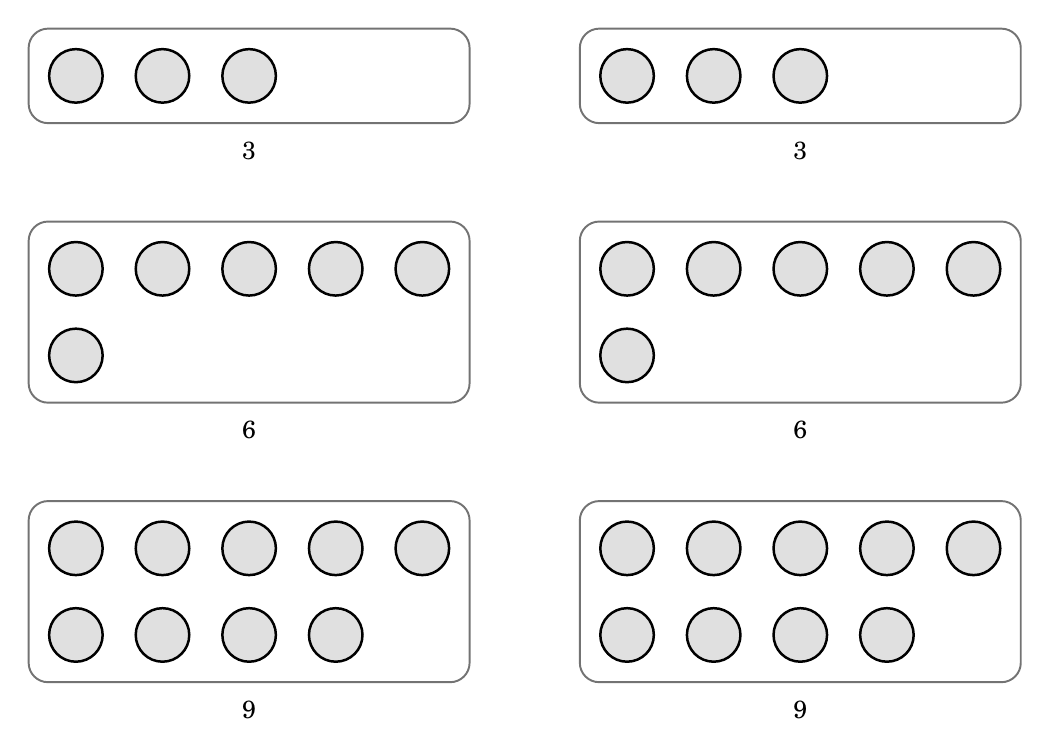
\begin{tikzpicture}
\draw[black!55,line width=0.7pt,rounded corners=7pt] (0.000,0.000) rectangle (5.600,-1.200);
\draw[fill=black!12,line width=0.9pt] (0.600,-0.600) circle (0.34);
\draw[fill=black!12,line width=0.9pt] (1.700,-0.600) circle (0.34);
\draw[fill=black!12,line width=0.9pt] (2.800,-0.600) circle (0.34);
\node[font=\small] at (2.800,-1.550) {3};
\draw[black!55,line width=0.7pt,rounded corners=7pt] (7.000,0.000) rectangle (12.600,-1.200);
\draw[fill=black!12,line width=0.9pt] (7.600,-0.600) circle (0.34);
\draw[fill=black!12,line width=0.9pt] (8.700,-0.600) circle (0.34);
\draw[fill=black!12,line width=0.9pt] (9.800,-0.600) circle (0.34);
\node[font=\small] at (9.800,-1.550) {3};
\draw[black!55,line width=0.7pt,rounded corners=7pt] (0.000,-2.450) rectangle (5.600,-4.750);
\draw[fill=black!12,line width=0.9pt] (0.600,-3.050) circle (0.34);
\draw[fill=black!12,line width=0.9pt] (1.700,-3.050) circle (0.34);
\draw[fill=black!12,line width=0.9pt] (2.800,-3.050) circle (0.34);
\draw[fill=black!12,line width=0.9pt] (3.900,-3.050) circle (0.34);
\draw[fill=black!12,line width=0.9pt] (5.000,-3.050) circle (0.34);
\draw[fill=black!12,line width=0.9pt] (0.600,-4.150) circle (0.34);
\node[font=\small] at (2.800,-5.100) {6};
\draw[black!55,line width=0.7pt,rounded corners=7pt] (7.000,-2.450) rectangle (12.600,-4.750);
\draw[fill=black!12,line width=0.9pt] (7.600,-3.050) circle (0.34);
\draw[fill=black!12,line width=0.9pt] (8.700,-3.050) circle (0.34);
\draw[fill=black!12,line width=0.9pt] (9.800,-3.050) circle (0.34);
\draw[fill=black!12,line width=0.9pt] (10.900,-3.050) circle (0.34);
\draw[fill=black!12,line width=0.9pt] (12.000,-3.050) circle (0.34);
\draw[fill=black!12,line width=0.9pt] (7.600,-4.150) circle (0.34);
\node[font=\small] at (9.800,-5.100) {6};
\draw[black!55,line width=0.7pt,rounded corners=7pt] (0.000,-6.000) rectangle (5.600,-8.300);
\draw[fill=black!12,line width=0.9pt] (0.600,-6.600) circle (0.34);
\draw[fill=black!12,line width=0.9pt] (1.700,-6.600) circle (0.34);
\draw[fill=black!12,line width=0.9pt] (2.800,-6.600) circle (0.34);
\draw[fill=black!12,line width=0.9pt] (3.900,-6.600) circle (0.34);
\draw[fill=black!12,line width=0.9pt] (5.000,-6.600) circle (0.34);
\draw[fill=black!12,line width=0.9pt] (0.600,-7.700) circle (0.34);
\draw[fill=black!12,line width=0.9pt] (1.700,-7.700) circle (0.34);
\draw[fill=black!12,line width=0.9pt] (2.800,-7.700) circle (0.34);
\draw[fill=black!12,line width=0.9pt] (3.900,-7.700) circle (0.34);
\node[font=\small] at (2.800,-8.650) {9};
\draw[black!55,line width=0.7pt,rounded corners=7pt] (7.000,-6.000) rectangle (12.600,-8.300);
\draw[fill=black!12,line width=0.9pt] (7.600,-6.600) circle (0.34);
\draw[fill=black!12,line width=0.9pt] (8.700,-6.600) circle (0.34);
\draw[fill=black!12,line width=0.9pt] (9.800,-6.600) circle (0.34);
\draw[fill=black!12,line width=0.9pt] (10.900,-6.600) circle (0.34);
\draw[fill=black!12,line width=0.9pt] (12.000,-6.600) circle (0.34);
\draw[fill=black!12,line width=0.9pt] (7.600,-7.700) circle (0.34);
\draw[fill=black!12,line width=0.9pt] (8.700,-7.700) circle (0.34);
\draw[fill=black!12,line width=0.9pt] (9.800,-7.700) circle (0.34);
\draw[fill=black!12,line width=0.9pt] (10.900,-7.700) circle (0.34);
\node[font=\small] at (9.800,-8.650) {9};
\end{tikzpicture}
\end{center}

\end{problem}
\begin{problem}
\prob{5} Ben always starts by taking 2 counters. Circle each pile where Ben can still be sure to win after that.
\begin{center}
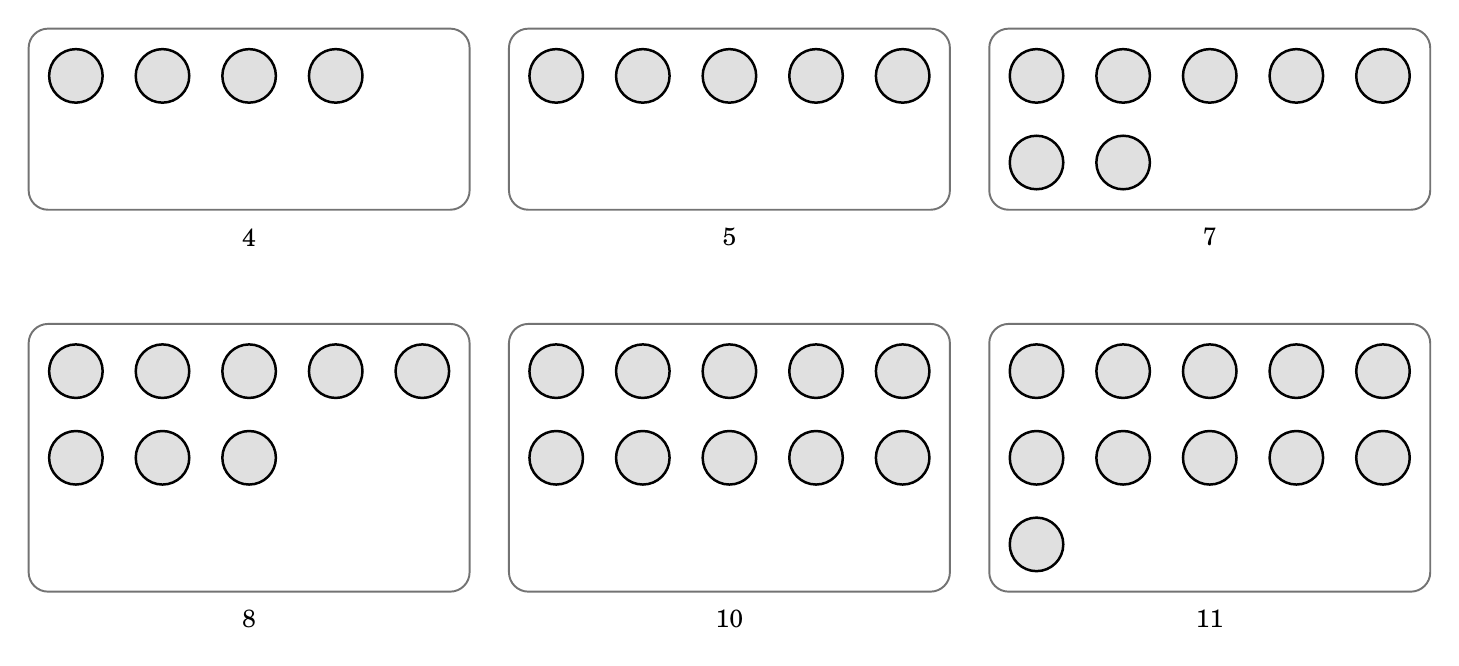
\begin{tikzpicture}
\draw[black!55,line width=0.7pt,rounded corners=7pt] (0.000,0.000) rectangle (5.600,-2.300);
\draw[fill=black!12,line width=0.9pt] (0.600,-0.600) circle (0.34);
\draw[fill=black!12,line width=0.9pt] (1.700,-0.600) circle (0.34);
\draw[fill=black!12,line width=0.9pt] (2.800,-0.600) circle (0.34);
\draw[fill=black!12,line width=0.9pt] (3.900,-0.600) circle (0.34);
\node[font=\small] at (2.800,-2.650) {4};
\draw[black!55,line width=0.7pt,rounded corners=7pt] (6.100,0.000) rectangle (11.700,-2.300);
\draw[fill=black!12,line width=0.9pt] (6.700,-0.600) circle (0.34);
\draw[fill=black!12,line width=0.9pt] (7.800,-0.600) circle (0.34);
\draw[fill=black!12,line width=0.9pt] (8.900,-0.600) circle (0.34);
\draw[fill=black!12,line width=0.9pt] (10.000,-0.600) circle (0.34);
\draw[fill=black!12,line width=0.9pt] (11.100,-0.600) circle (0.34);
\node[font=\small] at (8.900,-2.650) {5};
\draw[black!55,line width=0.7pt,rounded corners=7pt] (12.200,0.000) rectangle (17.800,-2.300);
\draw[fill=black!12,line width=0.9pt] (12.800,-0.600) circle (0.34);
\draw[fill=black!12,line width=0.9pt] (13.900,-0.600) circle (0.34);
\draw[fill=black!12,line width=0.9pt] (15.000,-0.600) circle (0.34);
\draw[fill=black!12,line width=0.9pt] (16.100,-0.600) circle (0.34);
\draw[fill=black!12,line width=0.9pt] (17.200,-0.600) circle (0.34);
\draw[fill=black!12,line width=0.9pt] (12.800,-1.700) circle (0.34);
\draw[fill=black!12,line width=0.9pt] (13.900,-1.700) circle (0.34);
\node[font=\small] at (15.000,-2.650) {7};
\draw[black!55,line width=0.7pt,rounded corners=7pt] (0.000,-3.750) rectangle (5.600,-7.150);
\draw[fill=black!12,line width=0.9pt] (0.600,-4.350) circle (0.34);
\draw[fill=black!12,line width=0.9pt] (1.700,-4.350) circle (0.34);
\draw[fill=black!12,line width=0.9pt] (2.800,-4.350) circle (0.34);
\draw[fill=black!12,line width=0.9pt] (3.900,-4.350) circle (0.34);
\draw[fill=black!12,line width=0.9pt] (5.000,-4.350) circle (0.34);
\draw[fill=black!12,line width=0.9pt] (0.600,-5.450) circle (0.34);
\draw[fill=black!12,line width=0.9pt] (1.700,-5.450) circle (0.34);
\draw[fill=black!12,line width=0.9pt] (2.800,-5.450) circle (0.34);
\node[font=\small] at (2.800,-7.500) {8};
\draw[black!55,line width=0.7pt,rounded corners=7pt] (6.100,-3.750) rectangle (11.700,-7.150);
\draw[fill=black!12,line width=0.9pt] (6.700,-4.350) circle (0.34);
\draw[fill=black!12,line width=0.9pt] (7.800,-4.350) circle (0.34);
\draw[fill=black!12,line width=0.9pt] (8.900,-4.350) circle (0.34);
\draw[fill=black!12,line width=0.9pt] (10.000,-4.350) circle (0.34);
\draw[fill=black!12,line width=0.9pt] (11.100,-4.350) circle (0.34);
\draw[fill=black!12,line width=0.9pt] (6.700,-5.450) circle (0.34);
\draw[fill=black!12,line width=0.9pt] (7.800,-5.450) circle (0.34);
\draw[fill=black!12,line width=0.9pt] (8.900,-5.450) circle (0.34);
\draw[fill=black!12,line width=0.9pt] (10.000,-5.450) circle (0.34);
\draw[fill=black!12,line width=0.9pt] (11.100,-5.450) circle (0.34);
\node[font=\small] at (8.900,-7.500) {10};
\draw[black!55,line width=0.7pt,rounded corners=7pt] (12.200,-3.750) rectangle (17.800,-7.150);
\draw[fill=black!12,line width=0.9pt] (12.800,-4.350) circle (0.34);
\draw[fill=black!12,line width=0.9pt] (13.900,-4.350) circle (0.34);
\draw[fill=black!12,line width=0.9pt] (15.000,-4.350) circle (0.34);
\draw[fill=black!12,line width=0.9pt] (16.100,-4.350) circle (0.34);
\draw[fill=black!12,line width=0.9pt] (17.200,-4.350) circle (0.34);
\draw[fill=black!12,line width=0.9pt] (12.800,-5.450) circle (0.34);
\draw[fill=black!12,line width=0.9pt] (13.900,-5.450) circle (0.34);
\draw[fill=black!12,line width=0.9pt] (15.000,-5.450) circle (0.34);
\draw[fill=black!12,line width=0.9pt] (16.100,-5.450) circle (0.34);
\draw[fill=black!12,line width=0.9pt] (17.200,-5.450) circle (0.34);
\draw[fill=black!12,line width=0.9pt] (12.800,-6.550) circle (0.34);
\node[font=\small] at (15.000,-7.500) {11};
\end{tikzpicture}
\end{center}

\end{problem}
\begin{problem}
\prob{6} Now each player may take 1, 2, or 3 counters on a turn. Put an X on every trap from 1 to 20.
\begin{center}
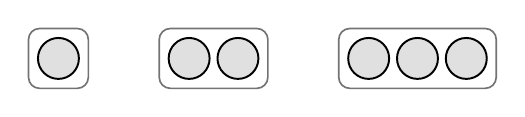
\begin{tikzpicture}
\draw[black!55,line width=0.6pt,rounded corners=4pt] (0.000,0) rectangle (0.760,-0.760);
\draw[fill=black!12,line width=0.7pt] (0.380,-0.380) circle (0.26);
\draw[black!55,line width=0.6pt,rounded corners=4pt] (1.660,0) rectangle (3.040,-0.760);
\draw[fill=black!12,line width=0.7pt] (2.040,-0.380) circle (0.26);
\draw[fill=black!12,line width=0.7pt] (2.660,-0.380) circle (0.26);
\draw[black!55,line width=0.6pt,rounded corners=4pt] (3.940,0) rectangle (5.940,-0.760);
\draw[fill=black!12,line width=0.7pt] (4.320,-0.380) circle (0.26);
\draw[fill=black!12,line width=0.7pt] (4.940,-0.380) circle (0.26);
\draw[fill=black!12,line width=0.7pt] (5.560,-0.380) circle (0.26);
\end{tikzpicture}
\end{center}
\vspace{-0.1cm}
\begin{center}
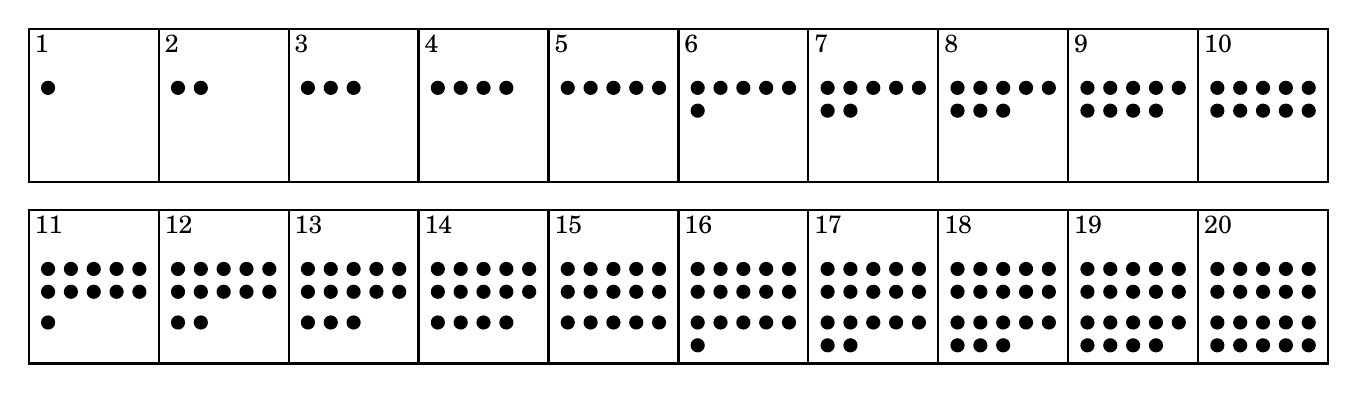
\begin{tikzpicture}
\draw[line width=0.8pt] (0.000,0.000) rectangle (1.650,-1.950);
\node[font=\small,anchor=north west,inner sep=2pt] at (0.000,0.000) {1};
\fill (0.245,-0.750) circle (0.09);
\draw[line width=0.8pt] (1.650,0.000) rectangle (3.300,-1.950);
\node[font=\small,anchor=north west,inner sep=2pt] at (1.650,0.000) {2};
\fill (1.895,-0.750) circle (0.09);
\fill (2.185,-0.750) circle (0.09);
\draw[line width=0.8pt] (3.300,0.000) rectangle (4.950,-1.950);
\node[font=\small,anchor=north west,inner sep=2pt] at (3.300,0.000) {3};
\fill (3.545,-0.750) circle (0.09);
\fill (3.835,-0.750) circle (0.09);
\fill (4.125,-0.750) circle (0.09);
\draw[line width=0.8pt] (4.950,0.000) rectangle (6.600,-1.950);
\node[font=\small,anchor=north west,inner sep=2pt] at (4.950,0.000) {4};
\fill (5.195,-0.750) circle (0.09);
\fill (5.485,-0.750) circle (0.09);
\fill (5.775,-0.750) circle (0.09);
\fill (6.065,-0.750) circle (0.09);
\draw[line width=0.8pt] (6.600,0.000) rectangle (8.250,-1.950);
\node[font=\small,anchor=north west,inner sep=2pt] at (6.600,0.000) {5};
\fill (6.845,-0.750) circle (0.09);
\fill (7.135,-0.750) circle (0.09);
\fill (7.425,-0.750) circle (0.09);
\fill (7.715,-0.750) circle (0.09);
\fill (8.005,-0.750) circle (0.09);
\draw[line width=0.8pt] (8.250,0.000) rectangle (9.900,-1.950);
\node[font=\small,anchor=north west,inner sep=2pt] at (8.250,0.000) {6};
\fill (8.495,-0.750) circle (0.09);
\fill (8.785,-0.750) circle (0.09);
\fill (9.075,-0.750) circle (0.09);
\fill (9.365,-0.750) circle (0.09);
\fill (9.655,-0.750) circle (0.09);
\fill (8.495,-1.040) circle (0.09);
\draw[line width=0.8pt] (9.900,0.000) rectangle (11.550,-1.950);
\node[font=\small,anchor=north west,inner sep=2pt] at (9.900,0.000) {7};
\fill (10.145,-0.750) circle (0.09);
\fill (10.435,-0.750) circle (0.09);
\fill (10.725,-0.750) circle (0.09);
\fill (11.015,-0.750) circle (0.09);
\fill (11.305,-0.750) circle (0.09);
\fill (10.145,-1.040) circle (0.09);
\fill (10.435,-1.040) circle (0.09);
\draw[line width=0.8pt] (11.550,0.000) rectangle (13.200,-1.950);
\node[font=\small,anchor=north west,inner sep=2pt] at (11.550,0.000) {8};
\fill (11.795,-0.750) circle (0.09);
\fill (12.085,-0.750) circle (0.09);
\fill (12.375,-0.750) circle (0.09);
\fill (12.665,-0.750) circle (0.09);
\fill (12.955,-0.750) circle (0.09);
\fill (11.795,-1.040) circle (0.09);
\fill (12.085,-1.040) circle (0.09);
\fill (12.375,-1.040) circle (0.09);
\draw[line width=0.8pt] (13.200,0.000) rectangle (14.850,-1.950);
\node[font=\small,anchor=north west,inner sep=2pt] at (13.200,0.000) {9};
\fill (13.445,-0.750) circle (0.09);
\fill (13.735,-0.750) circle (0.09);
\fill (14.025,-0.750) circle (0.09);
\fill (14.315,-0.750) circle (0.09);
\fill (14.605,-0.750) circle (0.09);
\fill (13.445,-1.040) circle (0.09);
\fill (13.735,-1.040) circle (0.09);
\fill (14.025,-1.040) circle (0.09);
\fill (14.315,-1.040) circle (0.09);
\draw[line width=0.8pt] (14.850,0.000) rectangle (16.500,-1.950);
\node[font=\small,anchor=north west,inner sep=2pt] at (14.850,0.000) {10};
\fill (15.095,-0.750) circle (0.09);
\fill (15.385,-0.750) circle (0.09);
\fill (15.675,-0.750) circle (0.09);
\fill (15.965,-0.750) circle (0.09);
\fill (16.255,-0.750) circle (0.09);
\fill (15.095,-1.040) circle (0.09);
\fill (15.385,-1.040) circle (0.09);
\fill (15.675,-1.040) circle (0.09);
\fill (15.965,-1.040) circle (0.09);
\fill (16.255,-1.040) circle (0.09);
\draw[line width=0.8pt] (0.000,-2.300) rectangle (1.650,-4.250);
\node[font=\small,anchor=north west,inner sep=2pt] at (0.000,-2.300) {11};
\fill (0.245,-3.050) circle (0.09);
\fill (0.535,-3.050) circle (0.09);
\fill (0.825,-3.050) circle (0.09);
\fill (1.115,-3.050) circle (0.09);
\fill (1.405,-3.050) circle (0.09);
\fill (0.245,-3.340) circle (0.09);
\fill (0.535,-3.340) circle (0.09);
\fill (0.825,-3.340) circle (0.09);
\fill (1.115,-3.340) circle (0.09);
\fill (1.405,-3.340) circle (0.09);
\fill (0.245,-3.730) circle (0.09);
\draw[line width=0.8pt] (1.650,-2.300) rectangle (3.300,-4.250);
\node[font=\small,anchor=north west,inner sep=2pt] at (1.650,-2.300) {12};
\fill (1.895,-3.050) circle (0.09);
\fill (2.185,-3.050) circle (0.09);
\fill (2.475,-3.050) circle (0.09);
\fill (2.765,-3.050) circle (0.09);
\fill (3.055,-3.050) circle (0.09);
\fill (1.895,-3.340) circle (0.09);
\fill (2.185,-3.340) circle (0.09);
\fill (2.475,-3.340) circle (0.09);
\fill (2.765,-3.340) circle (0.09);
\fill (3.055,-3.340) circle (0.09);
\fill (1.895,-3.730) circle (0.09);
\fill (2.185,-3.730) circle (0.09);
\draw[line width=0.8pt] (3.300,-2.300) rectangle (4.950,-4.250);
\node[font=\small,anchor=north west,inner sep=2pt] at (3.300,-2.300) {13};
\fill (3.545,-3.050) circle (0.09);
\fill (3.835,-3.050) circle (0.09);
\fill (4.125,-3.050) circle (0.09);
\fill (4.415,-3.050) circle (0.09);
\fill (4.705,-3.050) circle (0.09);
\fill (3.545,-3.340) circle (0.09);
\fill (3.835,-3.340) circle (0.09);
\fill (4.125,-3.340) circle (0.09);
\fill (4.415,-3.340) circle (0.09);
\fill (4.705,-3.340) circle (0.09);
\fill (3.545,-3.730) circle (0.09);
\fill (3.835,-3.730) circle (0.09);
\fill (4.125,-3.730) circle (0.09);
\draw[line width=0.8pt] (4.950,-2.300) rectangle (6.600,-4.250);
\node[font=\small,anchor=north west,inner sep=2pt] at (4.950,-2.300) {14};
\fill (5.195,-3.050) circle (0.09);
\fill (5.485,-3.050) circle (0.09);
\fill (5.775,-3.050) circle (0.09);
\fill (6.065,-3.050) circle (0.09);
\fill (6.355,-3.050) circle (0.09);
\fill (5.195,-3.340) circle (0.09);
\fill (5.485,-3.340) circle (0.09);
\fill (5.775,-3.340) circle (0.09);
\fill (6.065,-3.340) circle (0.09);
\fill (6.355,-3.340) circle (0.09);
\fill (5.195,-3.730) circle (0.09);
\fill (5.485,-3.730) circle (0.09);
\fill (5.775,-3.730) circle (0.09);
\fill (6.065,-3.730) circle (0.09);
\draw[line width=0.8pt] (6.600,-2.300) rectangle (8.250,-4.250);
\node[font=\small,anchor=north west,inner sep=2pt] at (6.600,-2.300) {15};
\fill (6.845,-3.050) circle (0.09);
\fill (7.135,-3.050) circle (0.09);
\fill (7.425,-3.050) circle (0.09);
\fill (7.715,-3.050) circle (0.09);
\fill (8.005,-3.050) circle (0.09);
\fill (6.845,-3.340) circle (0.09);
\fill (7.135,-3.340) circle (0.09);
\fill (7.425,-3.340) circle (0.09);
\fill (7.715,-3.340) circle (0.09);
\fill (8.005,-3.340) circle (0.09);
\fill (6.845,-3.730) circle (0.09);
\fill (7.135,-3.730) circle (0.09);
\fill (7.425,-3.730) circle (0.09);
\fill (7.715,-3.730) circle (0.09);
\fill (8.005,-3.730) circle (0.09);
\draw[line width=0.8pt] (8.250,-2.300) rectangle (9.900,-4.250);
\node[font=\small,anchor=north west,inner sep=2pt] at (8.250,-2.300) {16};
\fill (8.495,-3.050) circle (0.09);
\fill (8.785,-3.050) circle (0.09);
\fill (9.075,-3.050) circle (0.09);
\fill (9.365,-3.050) circle (0.09);
\fill (9.655,-3.050) circle (0.09);
\fill (8.495,-3.340) circle (0.09);
\fill (8.785,-3.340) circle (0.09);
\fill (9.075,-3.340) circle (0.09);
\fill (9.365,-3.340) circle (0.09);
\fill (9.655,-3.340) circle (0.09);
\fill (8.495,-3.730) circle (0.09);
\fill (8.785,-3.730) circle (0.09);
\fill (9.075,-3.730) circle (0.09);
\fill (9.365,-3.730) circle (0.09);
\fill (9.655,-3.730) circle (0.09);
\fill (8.495,-4.020) circle (0.09);
\draw[line width=0.8pt] (9.900,-2.300) rectangle (11.550,-4.250);
\node[font=\small,anchor=north west,inner sep=2pt] at (9.900,-2.300) {17};
\fill (10.145,-3.050) circle (0.09);
\fill (10.435,-3.050) circle (0.09);
\fill (10.725,-3.050) circle (0.09);
\fill (11.015,-3.050) circle (0.09);
\fill (11.305,-3.050) circle (0.09);
\fill (10.145,-3.340) circle (0.09);
\fill (10.435,-3.340) circle (0.09);
\fill (10.725,-3.340) circle (0.09);
\fill (11.015,-3.340) circle (0.09);
\fill (11.305,-3.340) circle (0.09);
\fill (10.145,-3.730) circle (0.09);
\fill (10.435,-3.730) circle (0.09);
\fill (10.725,-3.730) circle (0.09);
\fill (11.015,-3.730) circle (0.09);
\fill (11.305,-3.730) circle (0.09);
\fill (10.145,-4.020) circle (0.09);
\fill (10.435,-4.020) circle (0.09);
\draw[line width=0.8pt] (11.550,-2.300) rectangle (13.200,-4.250);
\node[font=\small,anchor=north west,inner sep=2pt] at (11.550,-2.300) {18};
\fill (11.795,-3.050) circle (0.09);
\fill (12.085,-3.050) circle (0.09);
\fill (12.375,-3.050) circle (0.09);
\fill (12.665,-3.050) circle (0.09);
\fill (12.955,-3.050) circle (0.09);
\fill (11.795,-3.340) circle (0.09);
\fill (12.085,-3.340) circle (0.09);
\fill (12.375,-3.340) circle (0.09);
\fill (12.665,-3.340) circle (0.09);
\fill (12.955,-3.340) circle (0.09);
\fill (11.795,-3.730) circle (0.09);
\fill (12.085,-3.730) circle (0.09);
\fill (12.375,-3.730) circle (0.09);
\fill (12.665,-3.730) circle (0.09);
\fill (12.955,-3.730) circle (0.09);
\fill (11.795,-4.020) circle (0.09);
\fill (12.085,-4.020) circle (0.09);
\fill (12.375,-4.020) circle (0.09);
\draw[line width=0.8pt] (13.200,-2.300) rectangle (14.850,-4.250);
\node[font=\small,anchor=north west,inner sep=2pt] at (13.200,-2.300) {19};
\fill (13.445,-3.050) circle (0.09);
\fill (13.735,-3.050) circle (0.09);
\fill (14.025,-3.050) circle (0.09);
\fill (14.315,-3.050) circle (0.09);
\fill (14.605,-3.050) circle (0.09);
\fill (13.445,-3.340) circle (0.09);
\fill (13.735,-3.340) circle (0.09);
\fill (14.025,-3.340) circle (0.09);
\fill (14.315,-3.340) circle (0.09);
\fill (14.605,-3.340) circle (0.09);
\fill (13.445,-3.730) circle (0.09);
\fill (13.735,-3.730) circle (0.09);
\fill (14.025,-3.730) circle (0.09);
\fill (14.315,-3.730) circle (0.09);
\fill (14.605,-3.730) circle (0.09);
\fill (13.445,-4.020) circle (0.09);
\fill (13.735,-4.020) circle (0.09);
\fill (14.025,-4.020) circle (0.09);
\fill (14.315,-4.020) circle (0.09);
\draw[line width=0.8pt] (14.850,-2.300) rectangle (16.500,-4.250);
\node[font=\small,anchor=north west,inner sep=2pt] at (14.850,-2.300) {20};
\fill (15.095,-3.050) circle (0.09);
\fill (15.385,-3.050) circle (0.09);
\fill (15.675,-3.050) circle (0.09);
\fill (15.965,-3.050) circle (0.09);
\fill (16.255,-3.050) circle (0.09);
\fill (15.095,-3.340) circle (0.09);
\fill (15.385,-3.340) circle (0.09);
\fill (15.675,-3.340) circle (0.09);
\fill (15.965,-3.340) circle (0.09);
\fill (16.255,-3.340) circle (0.09);
\fill (15.095,-3.730) circle (0.09);
\fill (15.385,-3.730) circle (0.09);
\fill (15.675,-3.730) circle (0.09);
\fill (15.965,-3.730) circle (0.09);
\fill (16.255,-3.730) circle (0.09);
\fill (15.095,-4.020) circle (0.09);
\fill (15.385,-4.020) circle (0.09);
\fill (15.675,-4.020) circle (0.09);
\fill (15.965,-4.020) circle (0.09);
\fill (16.255,-4.020) circle (0.09);
\end{tikzpicture}
\end{center}

\end{problem}
\begin{problem}
\prob{7} Now there are two piles, and on your turn you take 1 or 2 counters from one pile. Would you rather go 1st or 2nd? Circle it.
\begin{center}
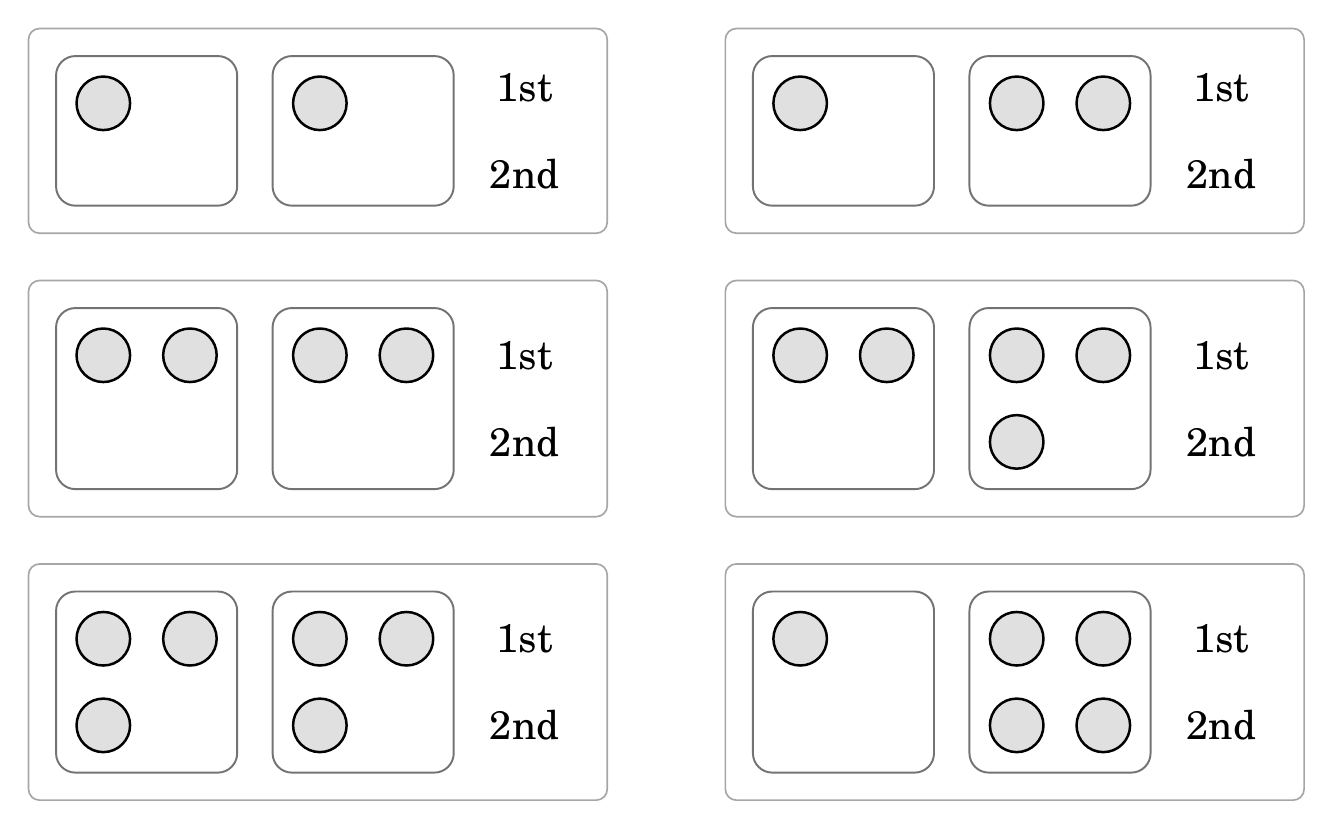
\begin{tikzpicture}
\draw[black!55,line width=0.7pt,rounded corners=7pt] (0.000,0.000) rectangle (2.300,-1.900);
\draw[fill=black!12,line width=0.9pt] (0.600,-0.600) circle (0.34);
\draw[black!55,line width=0.7pt,rounded corners=7pt] (2.750,0.000) rectangle (5.050,-1.900);
\draw[fill=black!12,line width=0.9pt] (3.350,-0.600) circle (0.34);
\node[font=\Large] at (5.950,-0.400) {1st};
\node[font=\Large] at (5.950,-1.500) {2nd};
\draw[black!35,line width=0.6pt,rounded corners=4pt] (-0.350,0.350) rectangle (7.000,-2.250);
\draw[black!55,line width=0.7pt,rounded corners=7pt] (8.850,0.000) rectangle (11.150,-1.900);
\draw[fill=black!12,line width=0.9pt] (9.450,-0.600) circle (0.34);
\draw[black!55,line width=0.7pt,rounded corners=7pt] (11.600,0.000) rectangle (13.900,-1.900);
\draw[fill=black!12,line width=0.9pt] (12.200,-0.600) circle (0.34);
\draw[fill=black!12,line width=0.9pt] (13.300,-0.600) circle (0.34);
\node[font=\Large] at (14.800,-0.400) {1st};
\node[font=\Large] at (14.800,-1.500) {2nd};
\draw[black!35,line width=0.6pt,rounded corners=4pt] (8.500,0.350) rectangle (15.850,-2.250);
\draw[black!55,line width=0.7pt,rounded corners=7pt] (0.000,-3.200) rectangle (2.300,-5.500);
\draw[fill=black!12,line width=0.9pt] (0.600,-3.800) circle (0.34);
\draw[fill=black!12,line width=0.9pt] (1.700,-3.800) circle (0.34);
\draw[black!55,line width=0.7pt,rounded corners=7pt] (2.750,-3.200) rectangle (5.050,-5.500);
\draw[fill=black!12,line width=0.9pt] (3.350,-3.800) circle (0.34);
\draw[fill=black!12,line width=0.9pt] (4.450,-3.800) circle (0.34);
\node[font=\Large] at (5.950,-3.800) {1st};
\node[font=\Large] at (5.950,-4.900) {2nd};
\draw[black!35,line width=0.6pt,rounded corners=4pt] (-0.350,-2.850) rectangle (7.000,-5.850);
\draw[black!55,line width=0.7pt,rounded corners=7pt] (8.850,-3.200) rectangle (11.150,-5.500);
\draw[fill=black!12,line width=0.9pt] (9.450,-3.800) circle (0.34);
\draw[fill=black!12,line width=0.9pt] (10.550,-3.800) circle (0.34);
\draw[black!55,line width=0.7pt,rounded corners=7pt] (11.600,-3.200) rectangle (13.900,-5.500);
\draw[fill=black!12,line width=0.9pt] (12.200,-3.800) circle (0.34);
\draw[fill=black!12,line width=0.9pt] (13.300,-3.800) circle (0.34);
\draw[fill=black!12,line width=0.9pt] (12.200,-4.900) circle (0.34);
\node[font=\Large] at (14.800,-3.800) {1st};
\node[font=\Large] at (14.800,-4.900) {2nd};
\draw[black!35,line width=0.6pt,rounded corners=4pt] (8.500,-2.850) rectangle (15.850,-5.850);
\draw[black!55,line width=0.7pt,rounded corners=7pt] (0.000,-6.800) rectangle (2.300,-9.100);
\draw[fill=black!12,line width=0.9pt] (0.600,-7.400) circle (0.34);
\draw[fill=black!12,line width=0.9pt] (1.700,-7.400) circle (0.34);
\draw[fill=black!12,line width=0.9pt] (0.600,-8.500) circle (0.34);
\draw[black!55,line width=0.7pt,rounded corners=7pt] (2.750,-6.800) rectangle (5.050,-9.100);
\draw[fill=black!12,line width=0.9pt] (3.350,-7.400) circle (0.34);
\draw[fill=black!12,line width=0.9pt] (4.450,-7.400) circle (0.34);
\draw[fill=black!12,line width=0.9pt] (3.350,-8.500) circle (0.34);
\node[font=\Large] at (5.950,-7.400) {1st};
\node[font=\Large] at (5.950,-8.500) {2nd};
\draw[black!35,line width=0.6pt,rounded corners=4pt] (-0.350,-6.450) rectangle (7.000,-9.450);
\draw[black!55,line width=0.7pt,rounded corners=7pt] (8.850,-6.800) rectangle (11.150,-9.100);
\draw[fill=black!12,line width=0.9pt] (9.450,-7.400) circle (0.34);
\draw[black!55,line width=0.7pt,rounded corners=7pt] (11.600,-6.800) rectangle (13.900,-9.100);
\draw[fill=black!12,line width=0.9pt] (12.200,-7.400) circle (0.34);
\draw[fill=black!12,line width=0.9pt] (13.300,-7.400) circle (0.34);
\draw[fill=black!12,line width=0.9pt] (12.200,-8.500) circle (0.34);
\draw[fill=black!12,line width=0.9pt] (13.300,-8.500) circle (0.34);
\node[font=\Large] at (14.800,-7.400) {1st};
\node[font=\Large] at (14.800,-8.500) {2nd};
\draw[black!35,line width=0.6pt,rounded corners=4pt] (8.500,-6.450) rectangle (15.850,-9.450);
\end{tikzpicture}
\end{center}

\end{problem}
\begin{problem}
\prob{8} Play the same game with two piles of 6, and go 2nd. Find a way to win every time, and show the adult.
\begin{center}
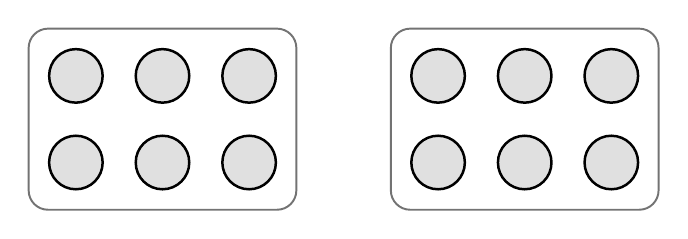
\begin{tikzpicture}
\draw[black!55,line width=0.7pt,rounded corners=7pt] (0.000,0.000) rectangle (3.400,-2.300);
\draw[fill=black!12,line width=0.9pt] (0.600,-0.600) circle (0.34);
\draw[fill=black!12,line width=0.9pt] (1.700,-0.600) circle (0.34);
\draw[fill=black!12,line width=0.9pt] (2.800,-0.600) circle (0.34);
\draw[fill=black!12,line width=0.9pt] (0.600,-1.700) circle (0.34);
\draw[fill=black!12,line width=0.9pt] (1.700,-1.700) circle (0.34);
\draw[fill=black!12,line width=0.9pt] (2.800,-1.700) circle (0.34);
\draw[black!55,line width=0.7pt,rounded corners=7pt] (4.600,0.000) rectangle (8.000,-2.300);
\draw[fill=black!12,line width=0.9pt] (5.200,-0.600) circle (0.34);
\draw[fill=black!12,line width=0.9pt] (6.300,-0.600) circle (0.34);
\draw[fill=black!12,line width=0.9pt] (7.400,-0.600) circle (0.34);
\draw[fill=black!12,line width=0.9pt] (5.200,-1.700) circle (0.34);
\draw[fill=black!12,line width=0.9pt] (6.300,-1.700) circle (0.34);
\draw[fill=black!12,line width=0.9pt] (7.400,-1.700) circle (0.34);
\end{tikzpicture}
\end{center}

\end{problem}
\begin{problem}
\prob{9} Now there is one pile, and each player may take 1 or 3 counters. Circle what you take to be sure to win, and cross out each trap.
\begin{center}
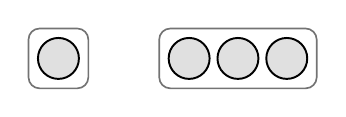
\begin{tikzpicture}
\draw[black!55,line width=0.6pt,rounded corners=4pt] (0.000,0) rectangle (0.760,-0.760);
\draw[fill=black!12,line width=0.7pt] (0.380,-0.380) circle (0.26);
\draw[black!55,line width=0.6pt,rounded corners=4pt] (1.660,0) rectangle (3.660,-0.760);
\draw[fill=black!12,line width=0.7pt] (2.040,-0.380) circle (0.26);
\draw[fill=black!12,line width=0.7pt] (2.660,-0.380) circle (0.26);
\draw[fill=black!12,line width=0.7pt] (3.280,-0.380) circle (0.26);
\end{tikzpicture}
\end{center}
\vspace{-0.1cm}
\begin{center}
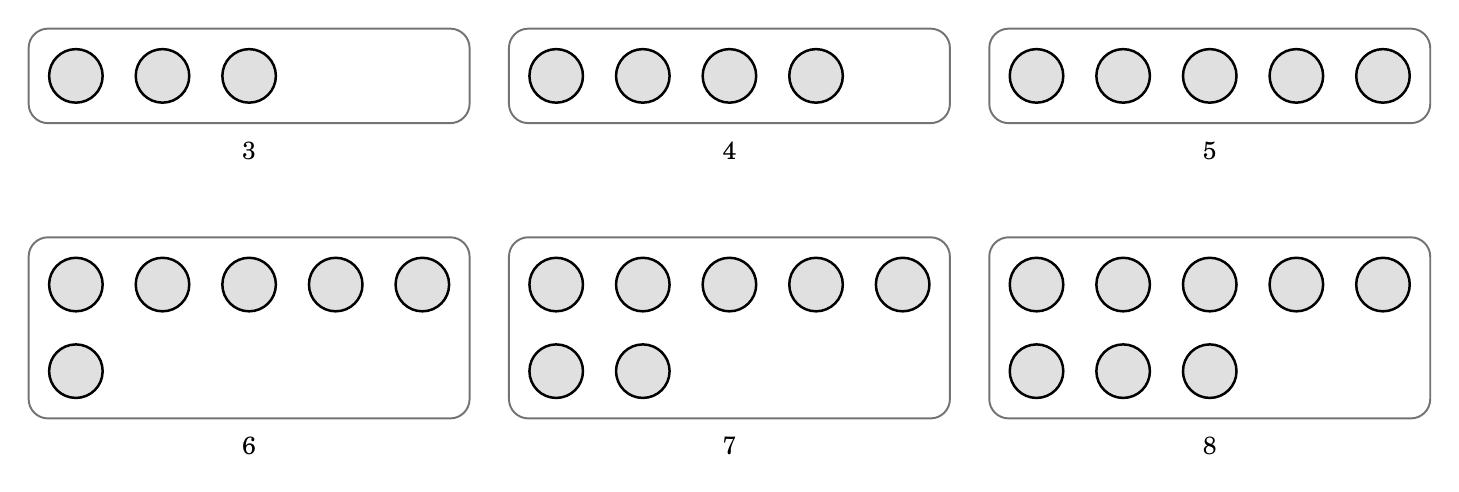
\begin{tikzpicture}
\draw[black!55,line width=0.7pt,rounded corners=7pt] (0.000,0.000) rectangle (5.600,-1.200);
\draw[fill=black!12,line width=0.9pt] (0.600,-0.600) circle (0.34);
\draw[fill=black!12,line width=0.9pt] (1.700,-0.600) circle (0.34);
\draw[fill=black!12,line width=0.9pt] (2.800,-0.600) circle (0.34);
\node[font=\small] at (2.800,-1.550) {3};
\draw[black!55,line width=0.7pt,rounded corners=7pt] (6.100,0.000) rectangle (11.700,-1.200);
\draw[fill=black!12,line width=0.9pt] (6.700,-0.600) circle (0.34);
\draw[fill=black!12,line width=0.9pt] (7.800,-0.600) circle (0.34);
\draw[fill=black!12,line width=0.9pt] (8.900,-0.600) circle (0.34);
\draw[fill=black!12,line width=0.9pt] (10.000,-0.600) circle (0.34);
\node[font=\small] at (8.900,-1.550) {4};
\draw[black!55,line width=0.7pt,rounded corners=7pt] (12.200,0.000) rectangle (17.800,-1.200);
\draw[fill=black!12,line width=0.9pt] (12.800,-0.600) circle (0.34);
\draw[fill=black!12,line width=0.9pt] (13.900,-0.600) circle (0.34);
\draw[fill=black!12,line width=0.9pt] (15.000,-0.600) circle (0.34);
\draw[fill=black!12,line width=0.9pt] (16.100,-0.600) circle (0.34);
\draw[fill=black!12,line width=0.9pt] (17.200,-0.600) circle (0.34);
\node[font=\small] at (15.000,-1.550) {5};
\draw[black!55,line width=0.7pt,rounded corners=7pt] (0.000,-2.650) rectangle (5.600,-4.950);
\draw[fill=black!12,line width=0.9pt] (0.600,-3.250) circle (0.34);
\draw[fill=black!12,line width=0.9pt] (1.700,-3.250) circle (0.34);
\draw[fill=black!12,line width=0.9pt] (2.800,-3.250) circle (0.34);
\draw[fill=black!12,line width=0.9pt] (3.900,-3.250) circle (0.34);
\draw[fill=black!12,line width=0.9pt] (5.000,-3.250) circle (0.34);
\draw[fill=black!12,line width=0.9pt] (0.600,-4.350) circle (0.34);
\node[font=\small] at (2.800,-5.300) {6};
\draw[black!55,line width=0.7pt,rounded corners=7pt] (6.100,-2.650) rectangle (11.700,-4.950);
\draw[fill=black!12,line width=0.9pt] (6.700,-3.250) circle (0.34);
\draw[fill=black!12,line width=0.9pt] (7.800,-3.250) circle (0.34);
\draw[fill=black!12,line width=0.9pt] (8.900,-3.250) circle (0.34);
\draw[fill=black!12,line width=0.9pt] (10.000,-3.250) circle (0.34);
\draw[fill=black!12,line width=0.9pt] (11.100,-3.250) circle (0.34);
\draw[fill=black!12,line width=0.9pt] (6.700,-4.350) circle (0.34);
\draw[fill=black!12,line width=0.9pt] (7.800,-4.350) circle (0.34);
\node[font=\small] at (8.900,-5.300) {7};
\draw[black!55,line width=0.7pt,rounded corners=7pt] (12.200,-2.650) rectangle (17.800,-4.950);
\draw[fill=black!12,line width=0.9pt] (12.800,-3.250) circle (0.34);
\draw[fill=black!12,line width=0.9pt] (13.900,-3.250) circle (0.34);
\draw[fill=black!12,line width=0.9pt] (15.000,-3.250) circle (0.34);
\draw[fill=black!12,line width=0.9pt] (16.100,-3.250) circle (0.34);
\draw[fill=black!12,line width=0.9pt] (17.200,-3.250) circle (0.34);
\draw[fill=black!12,line width=0.9pt] (12.800,-4.350) circle (0.34);
\draw[fill=black!12,line width=0.9pt] (13.900,-4.350) circle (0.34);
\draw[fill=black!12,line width=0.9pt] (15.000,-4.350) circle (0.34);
\node[font=\small] at (15.000,-5.300) {8};
\end{tikzpicture}
\end{center}

\end{problem}
\begin{problem}
\prob{10} Now each player takes 1 or 2 counters again, and whoever takes the last counter loses. Put an X on every trap from 1 to 20.
\begin{center}
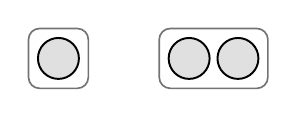
\begin{tikzpicture}
\draw[black!55,line width=0.6pt,rounded corners=4pt] (0.000,0) rectangle (0.760,-0.760);
\draw[fill=black!12,line width=0.7pt] (0.380,-0.380) circle (0.26);
\draw[black!55,line width=0.6pt,rounded corners=4pt] (1.660,0) rectangle (3.040,-0.760);
\draw[fill=black!12,line width=0.7pt] (2.040,-0.380) circle (0.26);
\draw[fill=black!12,line width=0.7pt] (2.660,-0.380) circle (0.26);
\end{tikzpicture}
\end{center}
\vspace{-0.1cm}
\begin{center}
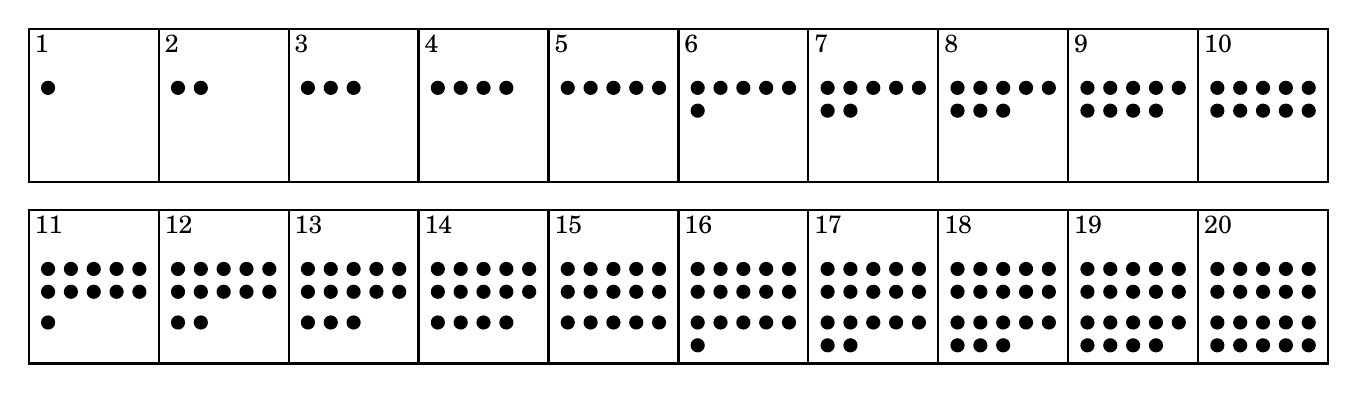
\begin{tikzpicture}
\draw[line width=0.8pt] (0.000,0.000) rectangle (1.650,-1.950);
\node[font=\small,anchor=north west,inner sep=2pt] at (0.000,0.000) {1};
\fill (0.245,-0.750) circle (0.09);
\draw[line width=0.8pt] (1.650,0.000) rectangle (3.300,-1.950);
\node[font=\small,anchor=north west,inner sep=2pt] at (1.650,0.000) {2};
\fill (1.895,-0.750) circle (0.09);
\fill (2.185,-0.750) circle (0.09);
\draw[line width=0.8pt] (3.300,0.000) rectangle (4.950,-1.950);
\node[font=\small,anchor=north west,inner sep=2pt] at (3.300,0.000) {3};
\fill (3.545,-0.750) circle (0.09);
\fill (3.835,-0.750) circle (0.09);
\fill (4.125,-0.750) circle (0.09);
\draw[line width=0.8pt] (4.950,0.000) rectangle (6.600,-1.950);
\node[font=\small,anchor=north west,inner sep=2pt] at (4.950,0.000) {4};
\fill (5.195,-0.750) circle (0.09);
\fill (5.485,-0.750) circle (0.09);
\fill (5.775,-0.750) circle (0.09);
\fill (6.065,-0.750) circle (0.09);
\draw[line width=0.8pt] (6.600,0.000) rectangle (8.250,-1.950);
\node[font=\small,anchor=north west,inner sep=2pt] at (6.600,0.000) {5};
\fill (6.845,-0.750) circle (0.09);
\fill (7.135,-0.750) circle (0.09);
\fill (7.425,-0.750) circle (0.09);
\fill (7.715,-0.750) circle (0.09);
\fill (8.005,-0.750) circle (0.09);
\draw[line width=0.8pt] (8.250,0.000) rectangle (9.900,-1.950);
\node[font=\small,anchor=north west,inner sep=2pt] at (8.250,0.000) {6};
\fill (8.495,-0.750) circle (0.09);
\fill (8.785,-0.750) circle (0.09);
\fill (9.075,-0.750) circle (0.09);
\fill (9.365,-0.750) circle (0.09);
\fill (9.655,-0.750) circle (0.09);
\fill (8.495,-1.040) circle (0.09);
\draw[line width=0.8pt] (9.900,0.000) rectangle (11.550,-1.950);
\node[font=\small,anchor=north west,inner sep=2pt] at (9.900,0.000) {7};
\fill (10.145,-0.750) circle (0.09);
\fill (10.435,-0.750) circle (0.09);
\fill (10.725,-0.750) circle (0.09);
\fill (11.015,-0.750) circle (0.09);
\fill (11.305,-0.750) circle (0.09);
\fill (10.145,-1.040) circle (0.09);
\fill (10.435,-1.040) circle (0.09);
\draw[line width=0.8pt] (11.550,0.000) rectangle (13.200,-1.950);
\node[font=\small,anchor=north west,inner sep=2pt] at (11.550,0.000) {8};
\fill (11.795,-0.750) circle (0.09);
\fill (12.085,-0.750) circle (0.09);
\fill (12.375,-0.750) circle (0.09);
\fill (12.665,-0.750) circle (0.09);
\fill (12.955,-0.750) circle (0.09);
\fill (11.795,-1.040) circle (0.09);
\fill (12.085,-1.040) circle (0.09);
\fill (12.375,-1.040) circle (0.09);
\draw[line width=0.8pt] (13.200,0.000) rectangle (14.850,-1.950);
\node[font=\small,anchor=north west,inner sep=2pt] at (13.200,0.000) {9};
\fill (13.445,-0.750) circle (0.09);
\fill (13.735,-0.750) circle (0.09);
\fill (14.025,-0.750) circle (0.09);
\fill (14.315,-0.750) circle (0.09);
\fill (14.605,-0.750) circle (0.09);
\fill (13.445,-1.040) circle (0.09);
\fill (13.735,-1.040) circle (0.09);
\fill (14.025,-1.040) circle (0.09);
\fill (14.315,-1.040) circle (0.09);
\draw[line width=0.8pt] (14.850,0.000) rectangle (16.500,-1.950);
\node[font=\small,anchor=north west,inner sep=2pt] at (14.850,0.000) {10};
\fill (15.095,-0.750) circle (0.09);
\fill (15.385,-0.750) circle (0.09);
\fill (15.675,-0.750) circle (0.09);
\fill (15.965,-0.750) circle (0.09);
\fill (16.255,-0.750) circle (0.09);
\fill (15.095,-1.040) circle (0.09);
\fill (15.385,-1.040) circle (0.09);
\fill (15.675,-1.040) circle (0.09);
\fill (15.965,-1.040) circle (0.09);
\fill (16.255,-1.040) circle (0.09);
\draw[line width=0.8pt] (0.000,-2.300) rectangle (1.650,-4.250);
\node[font=\small,anchor=north west,inner sep=2pt] at (0.000,-2.300) {11};
\fill (0.245,-3.050) circle (0.09);
\fill (0.535,-3.050) circle (0.09);
\fill (0.825,-3.050) circle (0.09);
\fill (1.115,-3.050) circle (0.09);
\fill (1.405,-3.050) circle (0.09);
\fill (0.245,-3.340) circle (0.09);
\fill (0.535,-3.340) circle (0.09);
\fill (0.825,-3.340) circle (0.09);
\fill (1.115,-3.340) circle (0.09);
\fill (1.405,-3.340) circle (0.09);
\fill (0.245,-3.730) circle (0.09);
\draw[line width=0.8pt] (1.650,-2.300) rectangle (3.300,-4.250);
\node[font=\small,anchor=north west,inner sep=2pt] at (1.650,-2.300) {12};
\fill (1.895,-3.050) circle (0.09);
\fill (2.185,-3.050) circle (0.09);
\fill (2.475,-3.050) circle (0.09);
\fill (2.765,-3.050) circle (0.09);
\fill (3.055,-3.050) circle (0.09);
\fill (1.895,-3.340) circle (0.09);
\fill (2.185,-3.340) circle (0.09);
\fill (2.475,-3.340) circle (0.09);
\fill (2.765,-3.340) circle (0.09);
\fill (3.055,-3.340) circle (0.09);
\fill (1.895,-3.730) circle (0.09);
\fill (2.185,-3.730) circle (0.09);
\draw[line width=0.8pt] (3.300,-2.300) rectangle (4.950,-4.250);
\node[font=\small,anchor=north west,inner sep=2pt] at (3.300,-2.300) {13};
\fill (3.545,-3.050) circle (0.09);
\fill (3.835,-3.050) circle (0.09);
\fill (4.125,-3.050) circle (0.09);
\fill (4.415,-3.050) circle (0.09);
\fill (4.705,-3.050) circle (0.09);
\fill (3.545,-3.340) circle (0.09);
\fill (3.835,-3.340) circle (0.09);
\fill (4.125,-3.340) circle (0.09);
\fill (4.415,-3.340) circle (0.09);
\fill (4.705,-3.340) circle (0.09);
\fill (3.545,-3.730) circle (0.09);
\fill (3.835,-3.730) circle (0.09);
\fill (4.125,-3.730) circle (0.09);
\draw[line width=0.8pt] (4.950,-2.300) rectangle (6.600,-4.250);
\node[font=\small,anchor=north west,inner sep=2pt] at (4.950,-2.300) {14};
\fill (5.195,-3.050) circle (0.09);
\fill (5.485,-3.050) circle (0.09);
\fill (5.775,-3.050) circle (0.09);
\fill (6.065,-3.050) circle (0.09);
\fill (6.355,-3.050) circle (0.09);
\fill (5.195,-3.340) circle (0.09);
\fill (5.485,-3.340) circle (0.09);
\fill (5.775,-3.340) circle (0.09);
\fill (6.065,-3.340) circle (0.09);
\fill (6.355,-3.340) circle (0.09);
\fill (5.195,-3.730) circle (0.09);
\fill (5.485,-3.730) circle (0.09);
\fill (5.775,-3.730) circle (0.09);
\fill (6.065,-3.730) circle (0.09);
\draw[line width=0.8pt] (6.600,-2.300) rectangle (8.250,-4.250);
\node[font=\small,anchor=north west,inner sep=2pt] at (6.600,-2.300) {15};
\fill (6.845,-3.050) circle (0.09);
\fill (7.135,-3.050) circle (0.09);
\fill (7.425,-3.050) circle (0.09);
\fill (7.715,-3.050) circle (0.09);
\fill (8.005,-3.050) circle (0.09);
\fill (6.845,-3.340) circle (0.09);
\fill (7.135,-3.340) circle (0.09);
\fill (7.425,-3.340) circle (0.09);
\fill (7.715,-3.340) circle (0.09);
\fill (8.005,-3.340) circle (0.09);
\fill (6.845,-3.730) circle (0.09);
\fill (7.135,-3.730) circle (0.09);
\fill (7.425,-3.730) circle (0.09);
\fill (7.715,-3.730) circle (0.09);
\fill (8.005,-3.730) circle (0.09);
\draw[line width=0.8pt] (8.250,-2.300) rectangle (9.900,-4.250);
\node[font=\small,anchor=north west,inner sep=2pt] at (8.250,-2.300) {16};
\fill (8.495,-3.050) circle (0.09);
\fill (8.785,-3.050) circle (0.09);
\fill (9.075,-3.050) circle (0.09);
\fill (9.365,-3.050) circle (0.09);
\fill (9.655,-3.050) circle (0.09);
\fill (8.495,-3.340) circle (0.09);
\fill (8.785,-3.340) circle (0.09);
\fill (9.075,-3.340) circle (0.09);
\fill (9.365,-3.340) circle (0.09);
\fill (9.655,-3.340) circle (0.09);
\fill (8.495,-3.730) circle (0.09);
\fill (8.785,-3.730) circle (0.09);
\fill (9.075,-3.730) circle (0.09);
\fill (9.365,-3.730) circle (0.09);
\fill (9.655,-3.730) circle (0.09);
\fill (8.495,-4.020) circle (0.09);
\draw[line width=0.8pt] (9.900,-2.300) rectangle (11.550,-4.250);
\node[font=\small,anchor=north west,inner sep=2pt] at (9.900,-2.300) {17};
\fill (10.145,-3.050) circle (0.09);
\fill (10.435,-3.050) circle (0.09);
\fill (10.725,-3.050) circle (0.09);
\fill (11.015,-3.050) circle (0.09);
\fill (11.305,-3.050) circle (0.09);
\fill (10.145,-3.340) circle (0.09);
\fill (10.435,-3.340) circle (0.09);
\fill (10.725,-3.340) circle (0.09);
\fill (11.015,-3.340) circle (0.09);
\fill (11.305,-3.340) circle (0.09);
\fill (10.145,-3.730) circle (0.09);
\fill (10.435,-3.730) circle (0.09);
\fill (10.725,-3.730) circle (0.09);
\fill (11.015,-3.730) circle (0.09);
\fill (11.305,-3.730) circle (0.09);
\fill (10.145,-4.020) circle (0.09);
\fill (10.435,-4.020) circle (0.09);
\draw[line width=0.8pt] (11.550,-2.300) rectangle (13.200,-4.250);
\node[font=\small,anchor=north west,inner sep=2pt] at (11.550,-2.300) {18};
\fill (11.795,-3.050) circle (0.09);
\fill (12.085,-3.050) circle (0.09);
\fill (12.375,-3.050) circle (0.09);
\fill (12.665,-3.050) circle (0.09);
\fill (12.955,-3.050) circle (0.09);
\fill (11.795,-3.340) circle (0.09);
\fill (12.085,-3.340) circle (0.09);
\fill (12.375,-3.340) circle (0.09);
\fill (12.665,-3.340) circle (0.09);
\fill (12.955,-3.340) circle (0.09);
\fill (11.795,-3.730) circle (0.09);
\fill (12.085,-3.730) circle (0.09);
\fill (12.375,-3.730) circle (0.09);
\fill (12.665,-3.730) circle (0.09);
\fill (12.955,-3.730) circle (0.09);
\fill (11.795,-4.020) circle (0.09);
\fill (12.085,-4.020) circle (0.09);
\fill (12.375,-4.020) circle (0.09);
\draw[line width=0.8pt] (13.200,-2.300) rectangle (14.850,-4.250);
\node[font=\small,anchor=north west,inner sep=2pt] at (13.200,-2.300) {19};
\fill (13.445,-3.050) circle (0.09);
\fill (13.735,-3.050) circle (0.09);
\fill (14.025,-3.050) circle (0.09);
\fill (14.315,-3.050) circle (0.09);
\fill (14.605,-3.050) circle (0.09);
\fill (13.445,-3.340) circle (0.09);
\fill (13.735,-3.340) circle (0.09);
\fill (14.025,-3.340) circle (0.09);
\fill (14.315,-3.340) circle (0.09);
\fill (14.605,-3.340) circle (0.09);
\fill (13.445,-3.730) circle (0.09);
\fill (13.735,-3.730) circle (0.09);
\fill (14.025,-3.730) circle (0.09);
\fill (14.315,-3.730) circle (0.09);
\fill (14.605,-3.730) circle (0.09);
\fill (13.445,-4.020) circle (0.09);
\fill (13.735,-4.020) circle (0.09);
\fill (14.025,-4.020) circle (0.09);
\fill (14.315,-4.020) circle (0.09);
\draw[line width=0.8pt] (14.850,-2.300) rectangle (16.500,-4.250);
\node[font=\small,anchor=north west,inner sep=2pt] at (14.850,-2.300) {20};
\fill (15.095,-3.050) circle (0.09);
\fill (15.385,-3.050) circle (0.09);
\fill (15.675,-3.050) circle (0.09);
\fill (15.965,-3.050) circle (0.09);
\fill (16.255,-3.050) circle (0.09);
\fill (15.095,-3.340) circle (0.09);
\fill (15.385,-3.340) circle (0.09);
\fill (15.675,-3.340) circle (0.09);
\fill (15.965,-3.340) circle (0.09);
\fill (16.255,-3.340) circle (0.09);
\fill (15.095,-3.730) circle (0.09);
\fill (15.385,-3.730) circle (0.09);
\fill (15.675,-3.730) circle (0.09);
\fill (15.965,-3.730) circle (0.09);
\fill (16.255,-3.730) circle (0.09);
\fill (15.095,-4.020) circle (0.09);
\fill (15.385,-4.020) circle (0.09);
\fill (15.675,-4.020) circle (0.09);
\fill (15.965,-4.020) circle (0.09);
\fill (16.255,-4.020) circle (0.09);
\end{tikzpicture}
\end{center}

\end{problem}
\end{document}
